\section{System Design}

\subsection{System Overview}
Determining the overall design of the system was initially hard since it was not clear exactly how many subsystems would be needed to refine, evaluate and interface with the finite element solver (see section 5.4 on LISA, the selected solver), It was clear however that the overriding feature that most influenced the design was the iterative approach required in order to repeatedly refine and analyse the mesh. Within the main process loop the  key focus was to ensure that the design remained modular with well defined relationships between classes so that the methods for refining and analysing the mesh could easily be added or modified independently of one another as the project progressed. \\ 


\noindent
The system can be broken down into the following main tasks that form the overall process to be undertaken: \\ 

\noindent
\textbf{Generate Initial Model: } Using an initial input file generated by LISA or other CAD package which contains the initial FEM model. \\ 

\noindent
\textbf{Solve Initial Mesh: } To initially calculate the stress in each element of the FEM model (i.e. to solve it) the .liml file is provided to LISA before being input into the developed software so that refinement can occur. \\ 

\noindent
\textbf{Read Solver Output: } Read the stress data computed across the mesh from the output file received from LISA and build a class model which can easily be manipulated by the refinement strategies.\\ 

\noindent
\textbf{Apply Refinement Processes : } Apply both the stress and rules based  refinement process to improve the mesh such that on the subsequent iteration more stress is revealed. \\ 

\noindent
\textbf{Quality checks on Refined Mesh : } Check the quality of the elements generated by refinement and prepare a new .liml file for next iteration of stress calculation.\\

\noindent
The relationships between these stages of the process are further illustrated in figure 4 below which shows the overall solution.


\begin{figure}[H]
  \centerline{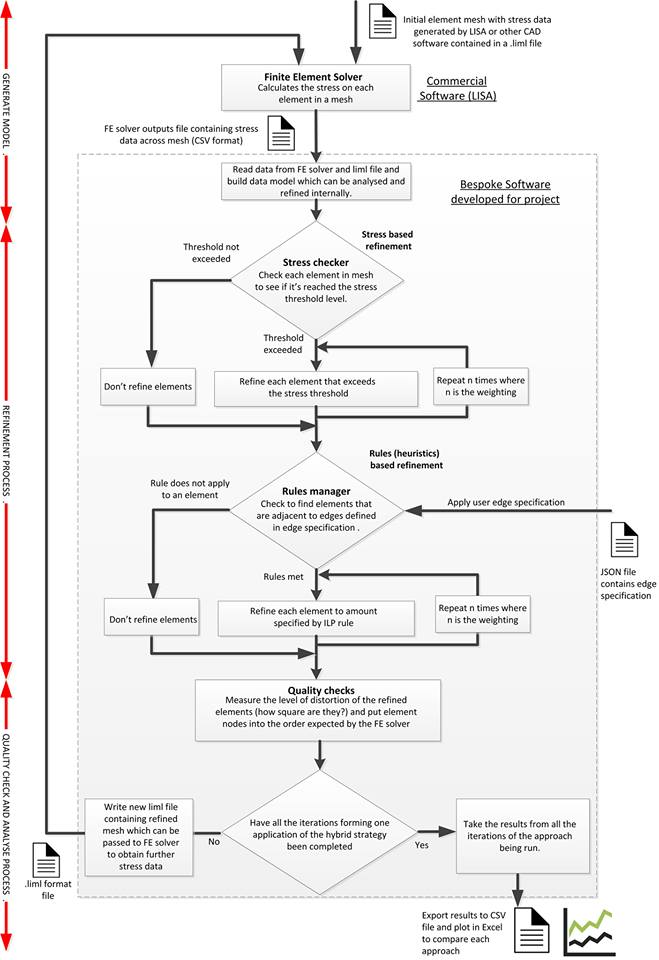
\includegraphics[width=150mm, scale=1]{../Graphics/ProcessDiagram}}
  \caption{High level Design of system/ refinement process}
  \label{fig:h-refinementImp}
\end{figure}



%\begin{figure}[H]
%  \centerline{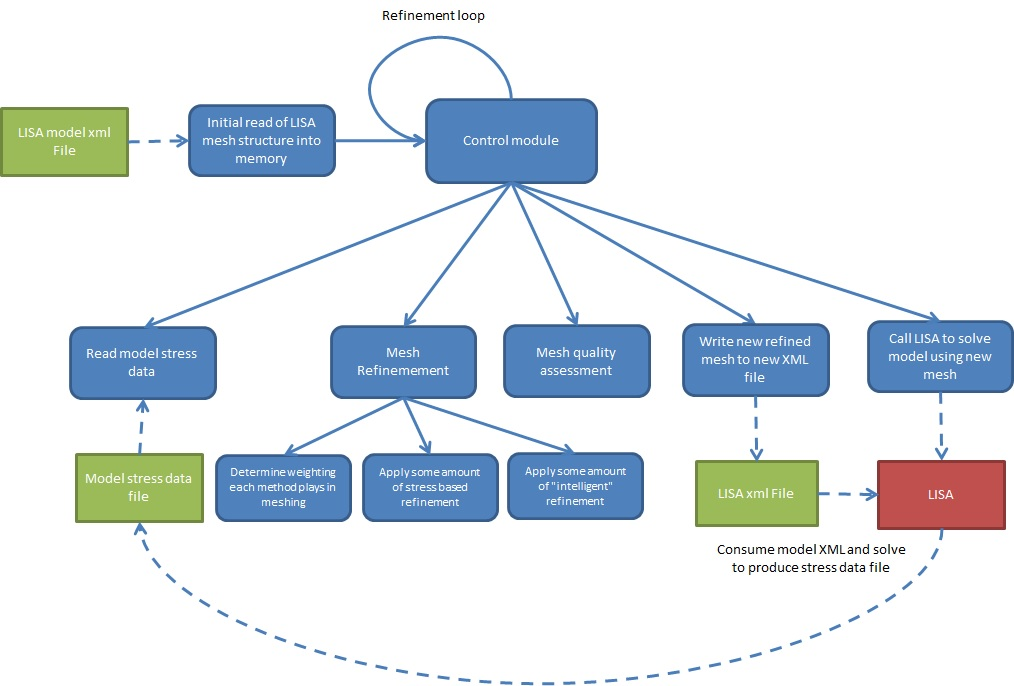
\includegraphics[width=150mm, %scale=1]{../Graphics/SystemDesignDiagram.jpeg}}
% \caption{High level design of the system with its different modules}
%  \label{fig:h-refinementImp}
%\end{figure}




\subsection{Modular Architecture}
The modular architecture was crucial for allowing meshing algorithms and quality metrics to be replaced as necessary. At best the quality of the output could only be predicted for each method before it was integrated into the system and executed in a range of different scenarios. To have tightly coupled these individual components would have rendered the overall system a failure in the event that any one of them failed. Instead the loose coupling of the architecture has enabled the system to be considered as more of a framework for testing the effects of combining different meshing approaches in order to generate a hybrid method.\\

\noindent
Although the system is highly modular It is still desirable to maintain an architecture hierarchy so that classes could be developed independently but easily integrated. Composition was therefore generally favoured over inheritance as a means of building the architecture. Static classes and methods were also used when needing to write utility functions that were required by multiple high level subsystems and therefore did not fit especially well into any particular one. Examples of these are generic vector algebra operations such as dot product, matrix determinant and calculating surface normals. \\ 

\noindent
At the highest level namespaces were used to break down the class groups appropriately, namespaces also naturally structured as folders within the Visual Studio (VS) solution explorer (see appendix F) which made navigating the project and finding components much easier as the system expanded in size.

%\subsection{Mesh improvement Loop}
%As with many optimisation problems the refinement process is driven iteratively through a loop. Within the main loop all %interfacing with LISA, Mesh refinement and analysis is conducted which results in an updated version of the model that can be %handed to the subsequent iteration.
\subsection{Third Party FE Application}
In order to demonstrate the potential feasibility of the hybrid approach it was important to first obtain a finite element solver which could be given a FE model containing data about forces, materials and the mesh structure and then execute the model programmatically so as to obtain stress results. \\ 

\noindent
A multitude of commercial FE tools exist with a wide range in both complexity and cost across all of them them.
Finite element software is typically very expensive however due to it having both a high development cost due to its complexity along with a relatively small and specialist user base. Tools used within industry such as ANSYS typically require a great deal of time in order to become proficient in their usage and can cost in excess of five thousand pounds a year for a single licence \cite{AnsysCost}. It was therefore important to find a tool which was both affordable while also powerful enough to demonstrate a working prototype of the re meshing method.
 
\subsection{LISA}
After reviewing several FE applications used within industry in addition to a variety of less well known ones used within academia and by hobbyists LISA  was selected as the solver application for which to implement  the systems prototypes. \\ 

\noindent
\textbf{Strengths: }LISA is a FE tool which allows the user to run models of up to 1300 element for free; This was beneficial in allowing me to experiment with the software and gauge the feasibility of my projects concept before requiring the full version for 299.99 Canadian dollars or £174.07. This purchase was only made however once at a stage in the project where each sub problem had been solved for small models containing less than 1300 elements and further work required testing with larger models. \\

\noindent
LISA also provides a GUI which allows visual inspection of the model and its mesh; this is particularly useful for observing the output of the meshing algorithms which can often provide a human with a much better understanding of how the method has performed and whether or not there are obvious bugs. in the implementation of the meshing procedures \\ 

\noindent
\textbf{Weaknesses: } Due to LISA’s simplicity it does not come with an extensive API allowing for easy programmatic use of its inbuilt features, however it is still possible to interface with LISA through less direct means \cite{LISAManual}. LISA models are stored in .liml files which use XML as a meta mark-up format. The model files contain all the information about the model including the materials used as well as loads and constraints and of course the mesh. It is therefore possible to manipulate a .liml file having parsed its contents before writing a new version of the file which LISA can be called to solve. In order to more easily alter the model it made sense to write a wrapper  for the .liml files to abstract and manipulate its content. \\ 


\subsection{Simulation Data Model}
Writing an API for LISA was the first stage of development for my project for which a design had to be considered. The API was crucial in order to program the more complex aspects using basic operations and to avoid having to regularly perform direct string manipulation of the input files when manipulating the model. \\

\noindent
When the first re-meshing iteration occurs the system needs to read the input .liml file into an equivalent class model which closely resembles the files schema. The model also contains the stress data from the previous iteration of the model. Diagrams for the model can be seen in figure 5 below. Each class in this model contains corresponding data and methods used to represent and manipulate the FE model. These methods are then used by each of the refinement approaches to easily alter the mesh in a controlled manner. Once the mesh has been refined however it is required to be assessed by the modules responsible for validating its quality before finally being written back to a .liml file for LISA to solve on the subsequent iteration. Designing the data model so that it closely resembled the LISA schema not only made the higher level programming less confusing but also made serialisation of the data back to .liml format much simpler  thus reducing the number of bugs arising from inconsistencies between different representations of the same data. \\

%\begin{figure}[h!]
%\centering

%\end{figure}



\begin{figure}[H]

\begin{subfigure}{.5\textwidth}
  \centering
  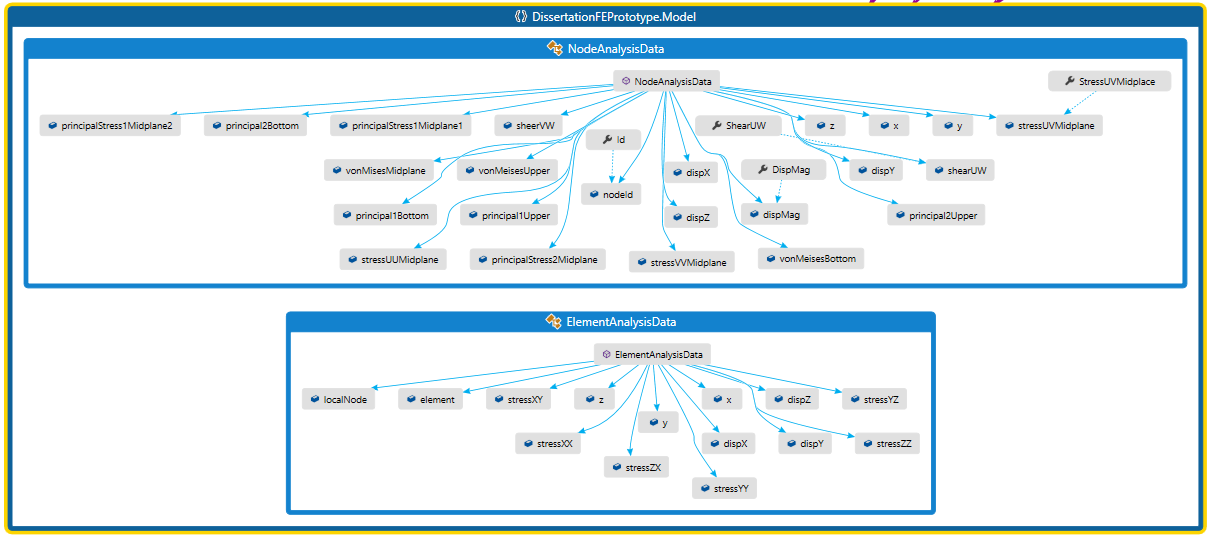
\includegraphics[width=0.9\linewidth]{../Graphics/DataModelStructure/Model.png}
  \caption{Model classes}
  \label{fig:sub1}
\end{subfigure}%
\begin{subfigure}{.5\textwidth}
  \centering
  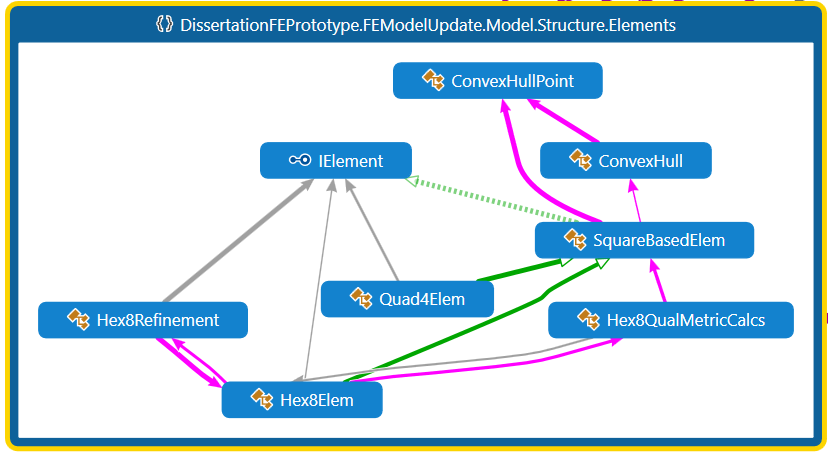
\includegraphics[width=0.9\linewidth]{../Graphics/DataModelStructure/Elements.png}
  \caption{Element Classes}
  \label{fig:sub2}
\end{subfigure}
\begin{subfigure}{.5\textwidth}
  \centering
  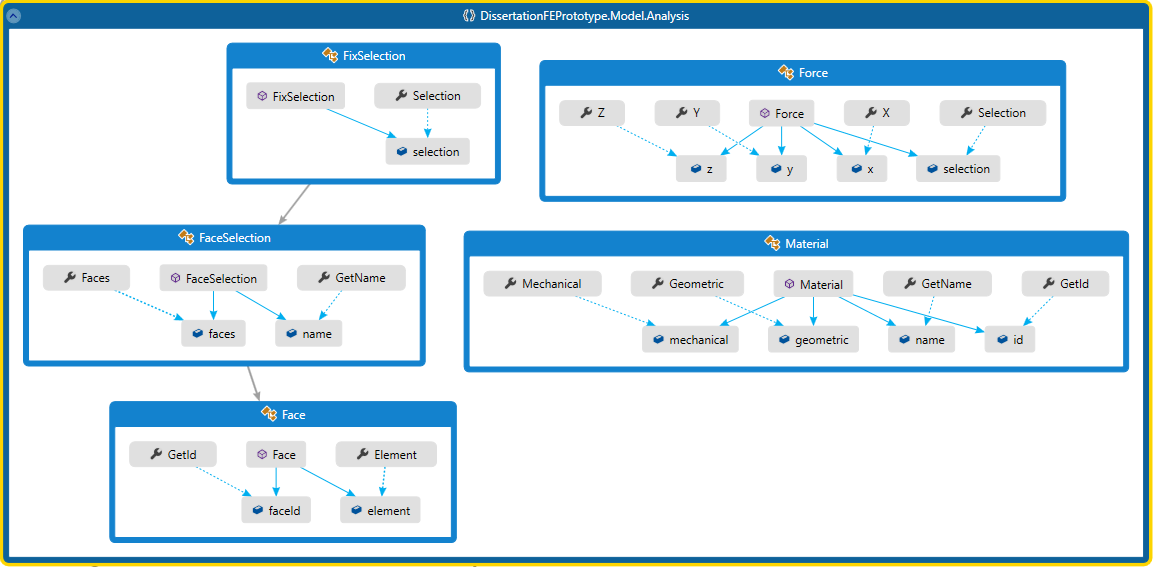
\includegraphics[width=0.9\linewidth]{../Graphics/DataModelStructure/ModelAnalysis.png}
  \caption{Model Analysis classes}
  \label{fig:sub1}
\end{subfigure}%
\begin{subfigure}{.5\textwidth}
  \centering
  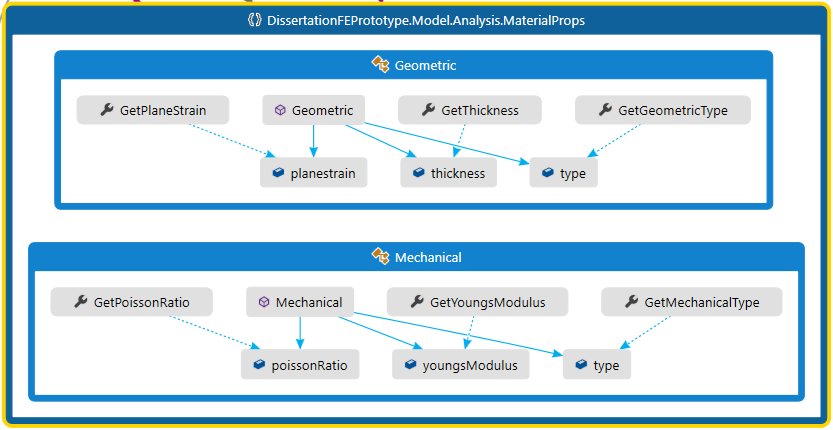
\includegraphics[width=0.9\linewidth]{../Graphics/DataModelStructure/MaterialProps.png}
  \caption{Material Property classes}
  \label{fig:sub2}
\end{subfigure}
\label{fig:test}
\caption{Class model to represent .liml file structure used by LISA}
\end{figure}


\noindent
One aspect of the data models design which greatly adds to the systems flexibility is the hierarchical design for representing the various element types. At the root of this structure is the IElement interface, all new element types must adhere to this in order for the various refinement methods to request refinement of an element using its class. Implementing the interface are a range of abstract classes such as ``SquareBasedElem" and ``TriangleBasedElem" These classes are designed to contain methods that are generally applicable for calculating metrics and re meshing individual elements where the elements fit this abstract category but their concrete implementation specifies their dimensionality and number of nodes, see figure 6 below. This is powerful since computing metrics and performing subdivision for a 3D element is simply a reduction using the code for a 2D element but over every face comprising the 3D one. Due to time limitations I was not able to implement the respective classes for triangle and line based elements, to see image representations of each element type within this class diagram refer to element types shown in appendix B.\\ 


%\pagestyle{empty}
\begin{landscape}

\begin{figure}[h]                                                   
  \centerline{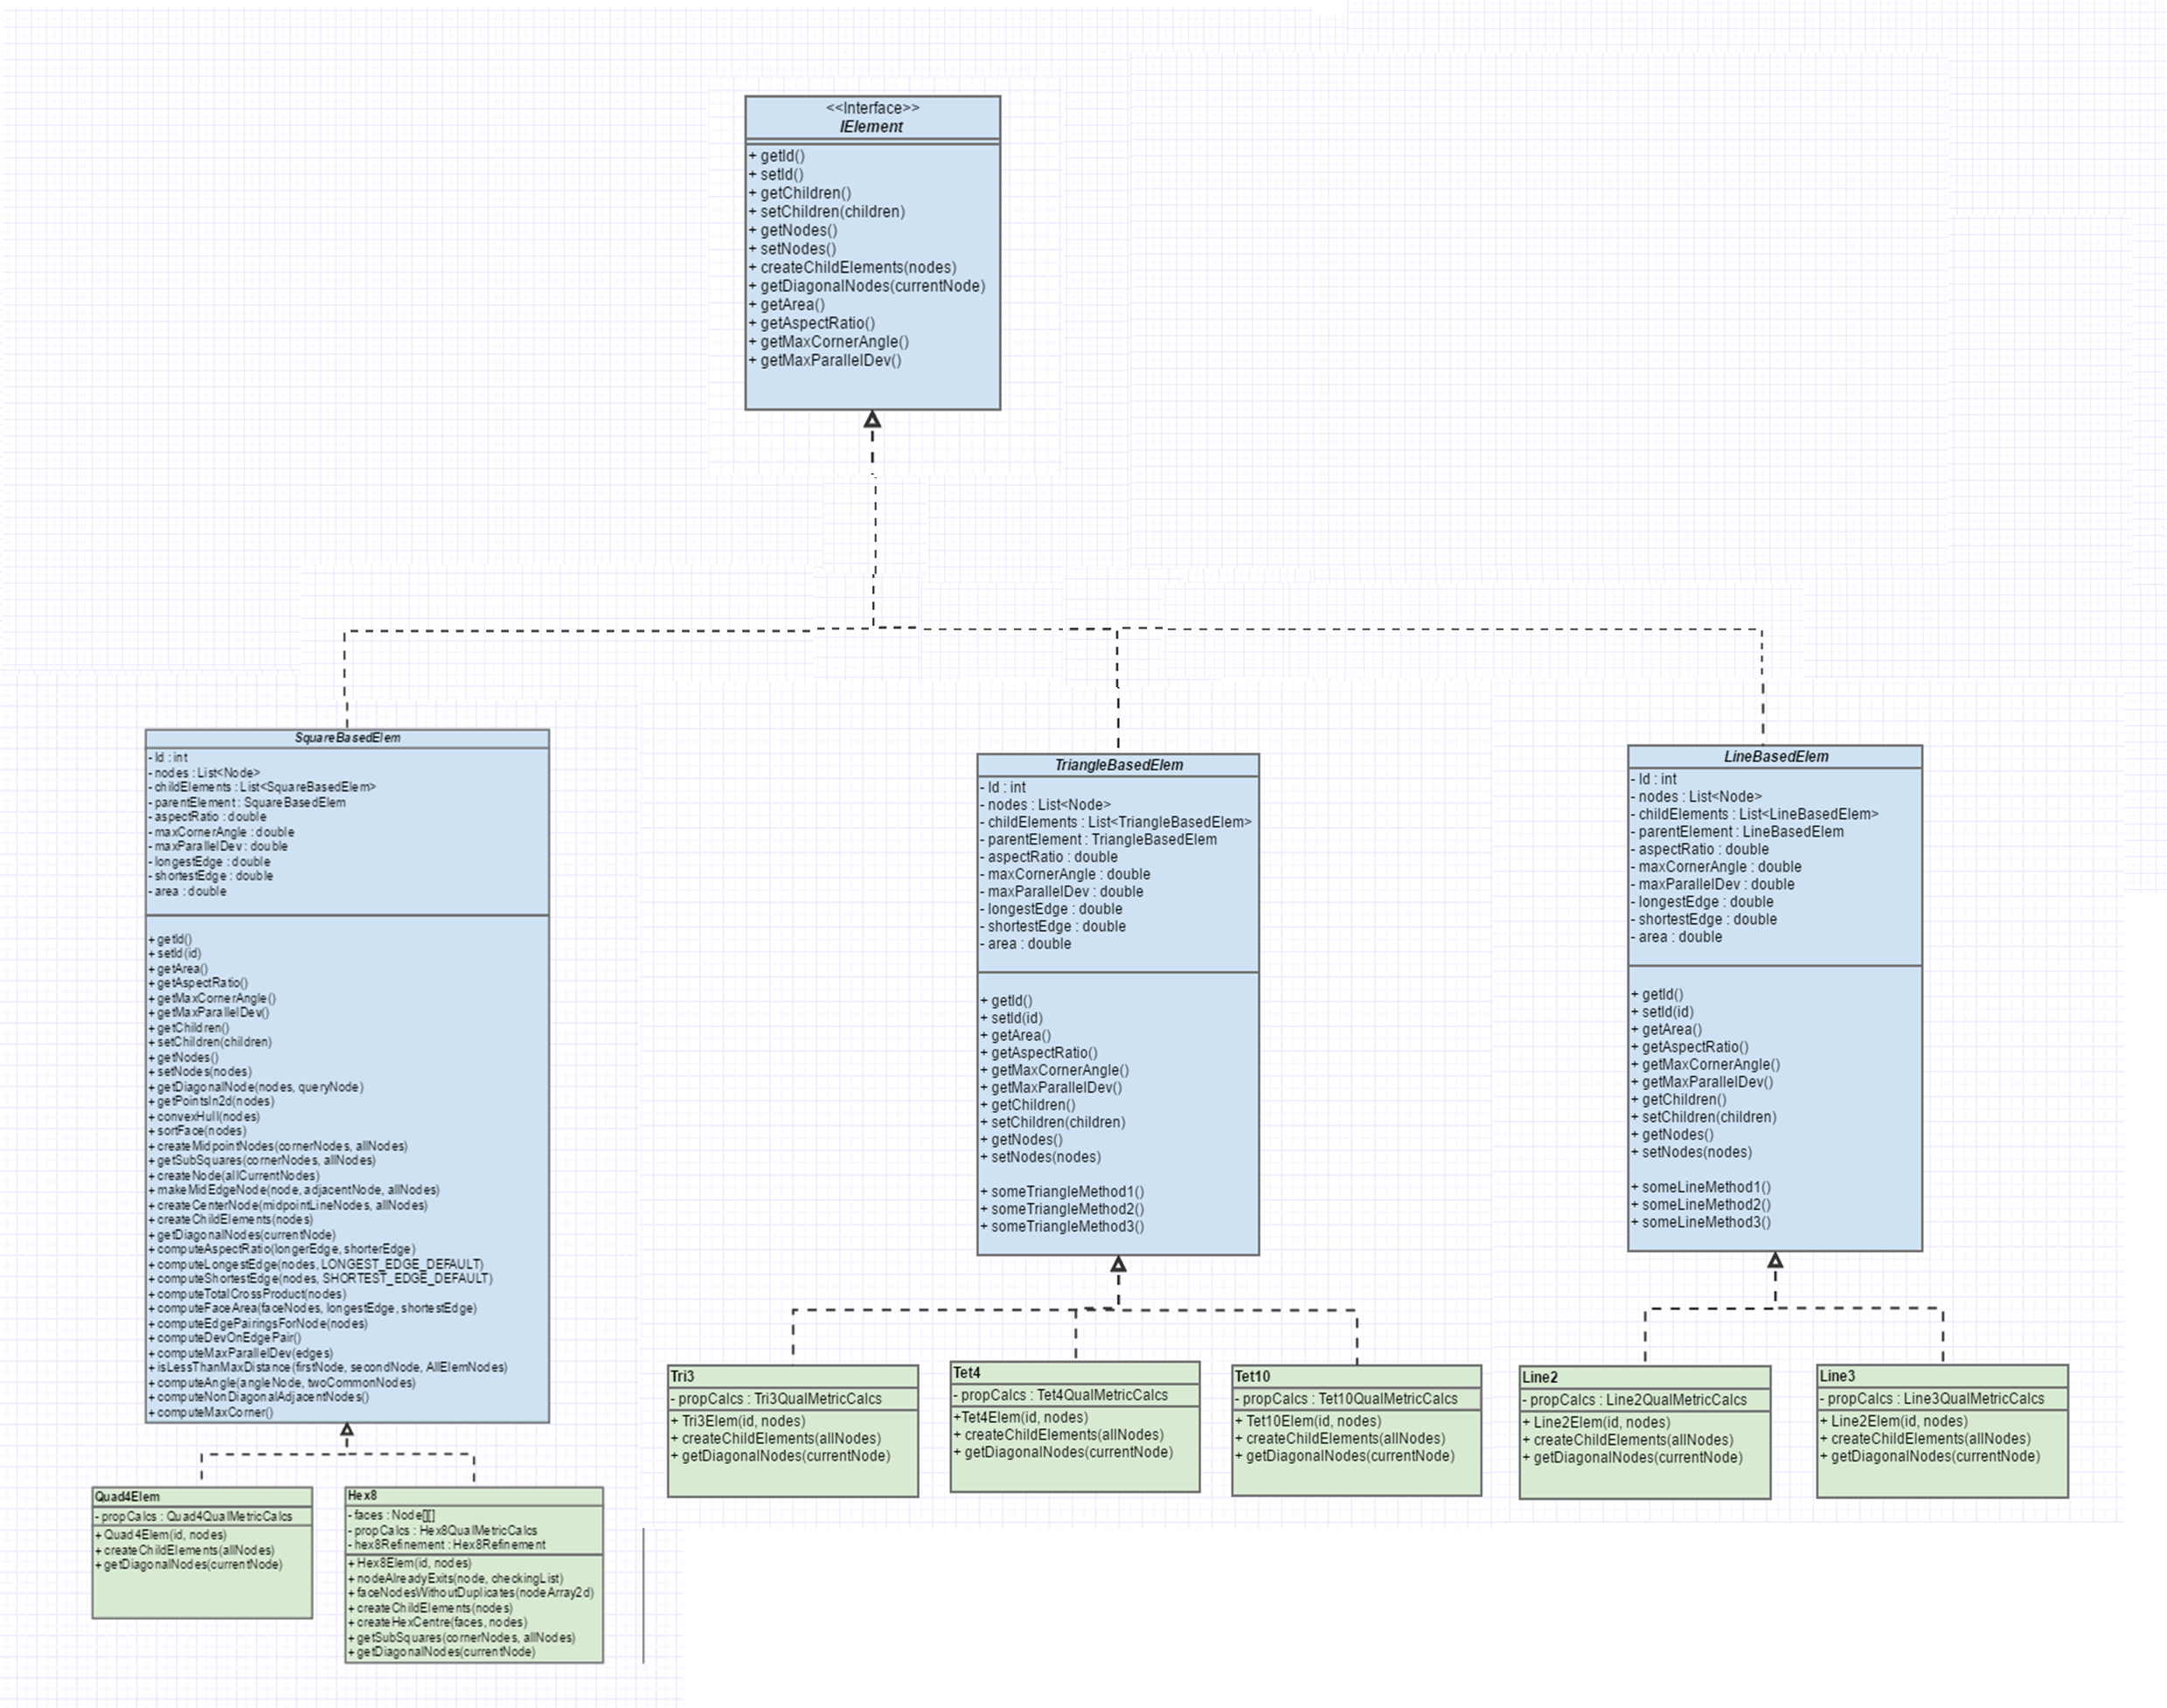
\includegraphics[width=220mm, scale=1]{../Graphics/ElementHigerarchyDiagram2.png}}
  \caption{Class diagram showing the hierarchy of element classification within the data model}
  \label{fig:h-refinementImp}
\end{figure}
\end{landscape}


\subsection{Remeshing Methods Approach}
When developing multiple meshing processes it was advantageous to break down and separate aspects of system functionality so that the system would be able to successfully incorporate new meshing procedures that may be added later. An FE mesh refinement system can be thought of as performing two distinct but related tasks: \\ 

\noindent
\textbf{Element Refinement: } How are elements going to be refined when it is known where it's best to refine within the mesh? \\

\noindent
\textbf{Meshing Strategy: } Which parts of the mesh are going to be refined? \\ 

\noindent
Both h and r refinement (described in section 3.1) fall under the first task and can be thought of as simply taking an argument from a higher level process about where they should mesh. \\

\noindent
By contrast stress refinement and the heuristic method that is also being used can be thought of as strategies. The goal of a strategy in this scenario is to maximise meshing in those areas where stress is likely to be high in advance of knowing the level of stress. Having computed the stress this also acts as the means by which to assess the quality of the strategy, that is being assessed by the system. Strategies are also much more general than subdivision processes and so it does not make sense to couple them to the subdivision functionality in any way. There is no reason that the same strategy shouldn't be used for a variety of meshes constructed out of different element types. The change in element shapes will however have an affect on how it is able to be subdivided. As a result the same subdivision code cannot be used to divide both a quadrilateral and a triangle, see appendix B for element types. \\ 


\noindent
The Design solution relating to this aspect of refinement was to abstract each of these concepts such that both strategies and element subdivision processes could be interchanged without any issues arising. Since subdivision is associated with specific elements the code for performing this task was encapsulated within a specific element class, from the Strategies perspective however it was important to be able to ask any type of element to subdivide itself. This was achieved through the design of an interface referred to in section 5.5 above as the IElement interface. Each type of element must implement this interface which exposes all the methods required for the controlling strategy to be able to refine the model in any chosen area. Using the interface the strategy can refine all elements it has selected as being beneficial for refinement by simply calling the elements createChildElements() method through the interface. This allowed any strategy to refine any type of element. \\ 

%These aspects of the design greatly improved code reuse and simplified the problem such that new high level approaches can easily be added without needing to consider how the underlying meshing takes place for models constructed using different elements. \\ 

\noindent
\textbf{Selecting a Subdivision Approach: }  Having reviewed both h-refinement \cite{HandPRefinements} and r-refinement \cite{RRefinement} as techniques for performing element subdivision it was concluded h-refinement was preferable due to its simplicity and widespread use despite typically being more computationally expensive than r-refinement \cite{HandPRefinements, RRefinement}. Another advantage of selecting h-refinement is how contained the approach is by only needing information about one particular element in order to refine it. By contrast r-refinement also needs to know about the state of the entire mesh which also contains the sizes and types of all the other elements, this  complicates an otherwise simple process of delegating the refinement task to specific elements in those regions of interest. Finally it is also not clear whether when implemented as part of a hybrid approach whether r-refinement would loop over and repeatedly swap the same elements when refining under two strategies simultaneously. This seems likely since each strategy asserts its own priorities for the method and will need to take elements from wherever else in the model there are lots of elements in order to further refine that area. \\ 


\noindent
After deciding to adopt h-refinement it was important to consider how new elements would be created and re integrated back into mesh structure. Subdividing elements recursively naturally forms a tree structure with an element creating additional smaller elements of the same type inside itself. The element type also largely determines the branching factor of the tree since most shapes naturally divide evenly into a specific number of smaller instances of themselves such that the shape of the original element is preserved. For example dividing a quadrilateral into four quarters results in each of the sub elements retaining the same aspect ratio as its parent. Alternatively dividing the same quadrilateral into two half's results in an aspect ratio twice as big, This is bad since the accuracy of the results produced by the solver for a mesh is highly dependent upon properties of each elements shape, see section 3.4 \cite{DittmerMeshQualityMet}. Once new elements have been created by the parent these new elements need to be registered within the main model. Initially the only element the model can see directly in its element list is the parent. This process involves updating the model reference such that the leaf nodes are added and the parent removed. To find the leafs a simple depth first search is performed and those elements with the structure which do not contain any children are added to the list. The final stage of the process is to assign unique id values to the elements so they can be referenced by LISA. Having constructed the list the first element is assigned the id of the parent and the parent destroyed, the following elements in the list are assigned the next available id values within the model. The subdivision process can be repeated arbitrarily many times before flattening the tree depending on the level of refinement desired. An example of the tree and the eventual flattened list can be seen below in figure 7. \\


\begin{figure}[!h]
  \centerline{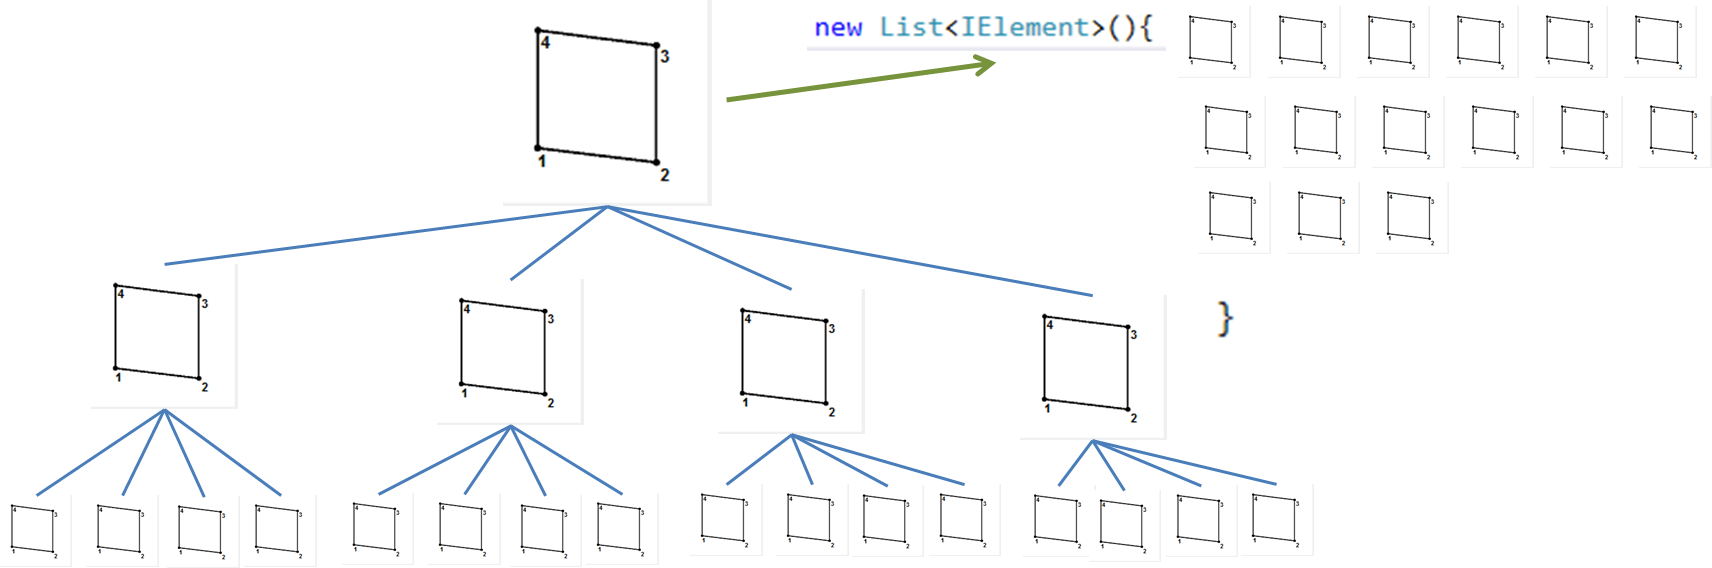
\includegraphics[width=150mm, scale=1]{../Graphics/ElemFlattening.png}}
  \caption{Process of flattening a refined element tree into a single list which can be handed back to LISA for processing}
  \label{fig:h-refinementImp}
\end{figure}


\noindent
\textbf{Stress Refinement: }
Designing a stress based refinement process involved three main steps, the specifics of which for my implementation are described under section 6.3. Firstly data needs to be obtained about the model stresses from the previous iteration, this is generated through execution of the mesh that is about to be refined. Once stress data is obtained along with a reference to the mesh it is possible to refine the mesh by using some evaluation function which takes both the mesh and the stress data and for every element in the mesh determines whether or not that element should be refined. selecting the threshold used by the evaluation function is perhaps the most important aspect of the design since since a high threshold, figure 8 shows stress refinement being applied across a simple four element mesh where the threshold is set as 7 \\ 

\noindent
\textbf{Heuristic Refinement: } 
Deciding on the second strategy by which to perform mesh refinement was perhaps the most significant design decision for the entire project. Having assessed a range of options, see section 3.3 it was realised that given the inherent complexity of the problem of developing a sophisticated AI method was going to be too time consuming. Dolsaks expert system \cite{DolsakPaper91, DolsakPaper94}, again reviewed in section 3.3 was therefore selected. Unlike some of the other approaches the literature also offered a straightforward implementation with clearly defined concepts and rules that  directly utilise the data already available within the LISA models. It's also important to note that the Dolsak used a machine learning technique and has published results that support the claims made of its capability, \cite{DolsakPaper91, DolsakPaper94, appOfILPToFEMeshDesign}. Use of this method as the second part of a hybrid approach ensures that the strengths of AI are Incorporated into the overall approach.  \\

\noindent
Unlike the stress refinement process which meshes purely based upon properties present in the current state of the model. The heuristic refinement process combines two sources of independent information when determining where best to mesh, these are the derived ILP rules and user defined edges. \\ 

\noindent
\textbf{Rules: } The rules produced by Golem, see section 3.3 are derived from training the ILP method using a series of meshes that were provided by by Dolsak \cite{DolsakPaper91, appOfILPToFEMeshDesign}. The rules are designed to take edges within the model as input and can decide how much meshing should be performed around those edges based on experience embedded within the rules by Golem through analysis of the training meshes. Ten of these rules which are provided within the research literature \cite{DolsakPaper91, appOfILPToFEMeshDesign} have been programmed into the system inside the ``RuleManager'' class within my system. \\ 

\noindent
\textbf{Edges: } Edges are the data used by the rules and are defined by engineers using the system. These engineers are likely to have some background knowledge of the component they are designing and so have the ability to assign some meta data to the edges, see section 6.4 and appendix E.\\ 


\noindent
Having been provided with a set of rules which can be applied to sets of edges it was important to design a mapping between the concept of an edge as described by Dolsak and the data model representing the FE mesh so the rules could drive the refinement. It was possible to approximate the concept of a smooth edge as a series of discrete node pairs within the mesh in order to form a path as a chain of nodes. This approach allows edges to be arbitrarily specified within the mesh structure using as much detail as was possible given the mesh's fidelity. Using this approach for defining edges in terms of the FE model meant that elements running along an edge that refinement needed to be made for could quickly be accessed by cross referencing the node Ids along the edge with those forming particular elements. \\ 


%as it offered a strategy system which is both simple to understand and implement with clear definitions in terms of concepts that already exist within the meshes

%Having evaluated a variety of approaches from the domains of AI it was concluded that the best approach for delivering a system capable of meeting the requirements and demonstrating effectiveness of a hybrid method would be an implementation of the heuristic expert system described by Dolsak. \\ 

\noindent
%One key strength of selecting this approach as the alternative method by which to mesh was clear separation of the underlying AI method from what had to be implemented. This not only meant that focus could be given towards the design, implementation and evaluation of the general purpose system but demonstrated that the meshing procedure can for the most part be interchanged depending on the specific type of finite element analysis. \\ 




\subsection{Input Files}
The system requires three basic input files which should be placed within a directory that is given to the program as a parameter, these files are:

\begin{itemize}
\item A structural model represented as a .liml file which LISA can solve.
\item An initial stress data file generated manually so the system has a starting point.
\item A JSON file containing important edges and associated meta data as identified by an engineer looking at the model.
\end{itemize}

An example of the content and format for each of these input files can be seen in appendix B


\subsection{Combining Methods to Form a Hybrid Approach}
Since each refinement method performed a discrete amount of subdivision every time it was called it made sense when developing a hybrid approach based on the two methods to define each potential hybrid as some weighted combination of the two methods. The simplest way to represent this appeared to be a two valued tuple containing the number of times each method should be applied for each iteration. One way to do this automatically would be to iterate through combinations of two integers up to some value k:

\[ \left\{ (HeuristicRefinementIterations, StressRefinementIterations) \,\middle|\, \, a,b \in \mathbb{N}\, \, a,b < k \right\} \]

\noindent
Using this weighting system each application of a method can be thought of as adding a depth of one to the trees of those elements that are affected by the rule as illustrated above in figure 7. Testing the hybrid weightings as different specifications meant it was also possible to improve the systems throughput by conducting evaluations simultaneously on different threads. When started each thread creates its own directory which it copies the three input files to and runs for its designating weighting configuration. \\

\noindent
Another key consideration when comparing the different meshing approaches was to establish what the value of weighting unit and thus allowing comparisons and evaluation for each of the hybrids as a weighting specification. Balance of the weightings was achieved at the start of the evaluation process through observing the increase in element count for the different heuristic methods when run individually. With the average increase in element count per iteration being calculated as 6\% of the model total in the case of the best sets of edge specifications (see section 7.6) The stress refinement threshold could then be configured so as only to mesh those elements within the 94th percentile within the model in terms of stress. \\

\noindent
An example of how both the stress and rule based refinement methods can be applied to the same mesh for a single solve iteration can be seen below in figure 8. Visual examples of how each of the meshing procedures affects the mesh can be seen in appendix J. Further detailed design details can be found in the section 6 covering the Software implementation. \\

\begin{figure}[H]
  \centerline{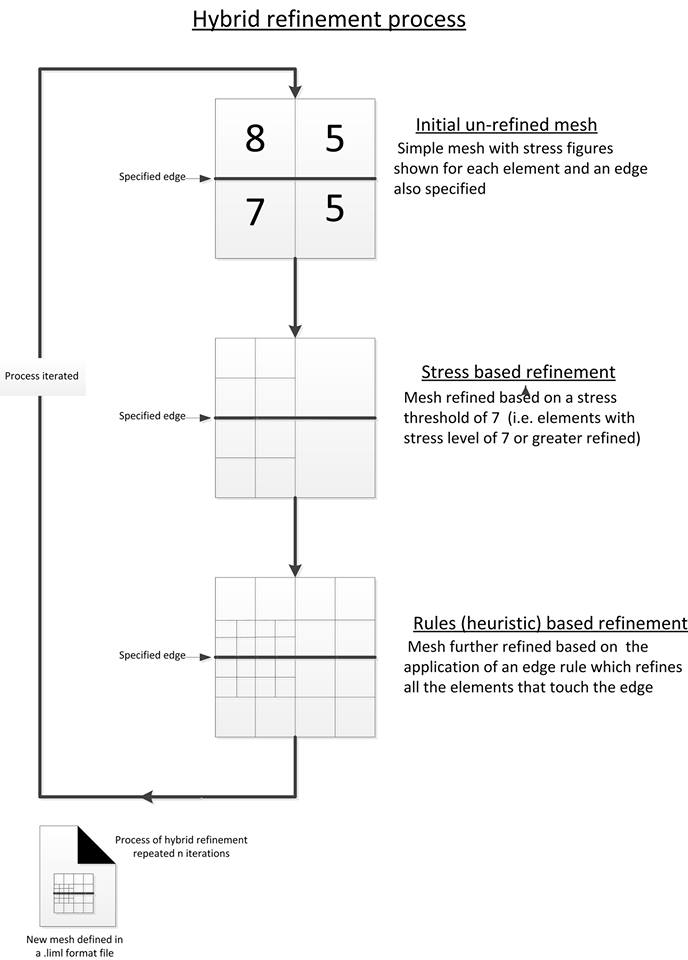
\includegraphics[width=150mm, scale=1]{../Graphics/HybridRefinement.jpg}}
  \caption{Applying both the stress and rule based refinement as part of one overall refinement iteration for a hybrid}
  \label{fig:h-refinementImp}
\end{figure}
